%%%%%%%%%%%%%%%%%%%%%%%%%%%%%%%%%%%%%%%%%
% Classicthesis Typographic Thesis
% LaTeX Template
% Version 1.4 (1/1/16)
%
% This template has been downloaded from:
% http://www.LaTeXTemplates.com
%
% Original author:
% André Miede (http://www.miede.de) with commenting modifications by:
% Vel (vel@LaTeXTemplates.com)
%
% License:
% GNU General Public License (v2)
%
% General Tips:
% 1) Make sure to edit the classicthesis-config.file
% 2) New enumeration (A., B., C., etc in small caps): \begin{aenumerate} \end{aenumerate}
% 3) For margin notes: \marginpar or \graffito{}
% 4) Do not use bold fonts in this style, it is designed around them
% 5) Use tables as in the examples
% 6) See classicthesis-preamble.sty for useful commands
%
%%%%%%%%%%%%%%%%%%%%%%%%%%%%%%%%%%%%%%%%%

%----------------------------------------------------------------------------------------
%	PACKAGES AND OTHER DOCUMENT CONFIGURATIONS
%----------------------------------------------------------------------------------------

\documentclass[
		twoside,openright,titlepage,numbers=noenddot,headinclude,%1headlines,
	 	footinclude=true,cleardoublepage=empty,
		dottedtoc, % Make page numbers in the table of contents flushed right with dots leading to them
		BCOR=5mm,paper=a4,fontsize=11pt, % Binding correction, paper type and font size
		ngerman,dutch, % Languages, change this to your language(s)
		]{scrreprt}

% Includes the file which contains all the document configurations and packages - make sure to edit this file
%%%%%%%%%%%%%%%%%%%%%%%%%%%%%%%%%%%%%%%%%
% Classicthesis Typographic Thesis
% Configuration File
%
% This file has been downloaded from:
% http://www.LaTeXTemplates.com
%
% Original author:
% André Miede (http://www.miede.de) with extensive commenting changes by:
% Vel (vel@LaTeXTemplates.com)
%
% License:
% GNU General Public License (v2)
%
% Important note:
% The main lines to change in this file are in the DOCUMENT VARIABLES
% section, the rest of the file is for advanced configuration.
%
%%%%%%%%%%%%%%%%%%%%%%%%%%%%%%%%%%%%%%%%%

%----------------------------------------------------------------------------------------
%	CHARACTER ENCODING
%----------------------------------------------------------------------------------------

\PassOptionsToPackage{utf8}{inputenc} % Set the encoding of your files. UTF-8 is the only sensible encoding nowadays. If you can't read äöüßáéçèê∂åëæƒÏ€ then change the encoding setting in your editor, not the line below. If your editor does not support utf8 use another editor!
\usepackage{inputenc}

%----------------------------------------------------------------------------------------
%	DOCUMENT VARIABLES
%	Fill in the lines below to enter your information into the thesis template
%	Each of the commands can be cited anywhere in the thesis
%----------------------------------------------------------------------------------------

% Remove drafting to get rid of the '[ Date - classicthesis version 4.0 ]' text at the bottom of every page
%\PassOptionsToPackage{eulerchapternumbers,listings,drafting, pdfspacing, subfig,beramono,eulermath,parts}{classicthesis}
% Available options: drafting parts nochapters linedheaders eulerchapternumbers beramono eulermath pdfspacing minionprospacing tocaligned dottedtoc manychapters listings floatperchapter subfig

\newcommand{\myTitle}{Analysing SOUP\xspace}
\newcommand{\mySubtitle}{Een weg naar veiligere software\xspace}
\newcommand{\myDegree}{Doktor-Ingenieur (Dr.-Ing.)\xspace}
\newcommand{\myName}{Bas Brunink\xspace}
\newcommand{\myFaculty}{FDMCI\xspace}
\newcommand{\myDepartment}{Software Engineering\xspace}
\newcommand{\myUni}{Hogeschool van Amsterdam\xspace}
\newcommand{\myHvABegeleider}{Fatih Caglayan}
\newcommand{\myLocation}{Amsterdam\xspace}
\newcommand{\myTime}{Februari 2022\xspace}
\newcommand{\myVersion}{version 1\xspace}

\newcommand{\myStagebegeleider}{Bas Breijer \xspace}
\newcommand{\myworkName}{Eaglescience\xspace}
\newcommand{\myworkAddress}{Naritaweg 12K\xspace}
\newcommand{\myworkPostcodeCity}{1043 BZ Amsterdam\xspace}


%----------------------------------------------------------------------------------------
%	USEFUL COMMANDS
%----------------------------------------------------------------------------------------

\newcommand{\ie}{i.\,e.}
\newcommand{\Ie}{I.\,e.}
\newcommand{\eg}{e.\,g.}
\newcommand{\Eg}{E.\,g.}

\newcounter{dummy} % Necessary for correct hyperlinks (to index, bib, etc.)
\providecommand{\mLyX}{L\kern-.1667em\lower.25em\hbox{Y}\kern-.125emX\@}
\newlength{\abcd} % for ab..z string length calculation

%----------------------------------------------------------------------------------------
%	PACKAGES
%----------------------------------------------------------------------------------------

\usepackage{lipsum} % Used for inserting dummy 'Lorem ipsum' text into the template

%------------------------------------------------

%\PassOptionsToPackage{ngerman,american}{babel}  % Change this to your language(s)
% Spanish languages need extra options in order to work with this template
%\PassOptionsToPackage{spanish,es-lcroman}{babel}
\usepackage{babel}

%------------------------------------------------

\usepackage{csquotes}
\PassOptionsToPackage{%
%backend=biber, % Instead of bibtex
backend=bibtex8,bibencoding=ascii,%
language=auto,%
%style=numeric-comp,%
style=authoryear-comp, % Author 1999, 2010
%bibstyle=authoryear,dashed=false, % dashed: substitute rep. author with ---
sorting=nyt, % name, year, title
maxbibnames=10, % default: 3, et al.
%backref=true,%
natbib=true % natbib compatibility mode (\citep and \citet still work)
}{biblatex}
\usepackage{biblatex}

 %------------------------------------------------

\PassOptionsToPackage{fleqn}{amsmath} % Math environments and more by the AMS
 \usepackage{amsmath}

 %------------------------------------------------

\PassOptionsToPackage{T1}{fontenc} % T2A for cyrillics
\usepackage{fontenc}

%------------------------------------------------

\usepackage{textcomp} % Fix warning with missing font shapes

%------------------------------------------------

\usepackage{scrhack} % Fix warnings when using KOMA with listings package

%------------------------------------------------

\usepackage{xspace} % To get the spacing after macros right

%------------------------------------------------

\usepackage{mparhack} % To get marginpar right

%------------------------------------------------

%\usepackage{fixltx2e} % Fixes some LaTeX stuff

%------------------------------------------------

\usepackage{url} %% fix for urls in cites

\PassOptionsToPackage{smaller}{acronym} % Include printonlyused in the first bracket to only show acronyms used in the text
\usepackage{acronym} % Nice macros for handling all acronyms in the thesis

%\renewcommand*{\acsfont}[1]{\textssc{#1}} % For MinionPro
\renewcommand*{\aclabelfont}[1]{\acsfont{#1}}

%------------------------------------------------

\PassOptionsToPackage{pdftex}{graphicx}
\usepackage{graphicx}

%----------------------------------------------------------------------------------------
%	FLOATS: TABLES, FIGURES AND CAPTIONS SETUP
%----------------------------------------------------------------------------------------

\usepackage{tabularx} % Better tables
\setlength{\extrarowheight}{3pt} % Increase table row height
\newcommand{\tableheadline}[1]{\multicolumn{1}{c}{\spacedlowsmallcaps{#1}}}
\newcommand{\myfloatalign}{\centering} % To be used with each float for alignment
\usepackage{caption}
\captionsetup{font=small}
\usepackage{subfig}

%----------------------------------------------------------------------------------------
%	CODE LISTINGS SETUP
%----------------------------------------------------------------------------------------

\usepackage{listings}
%\lstset{emph={trueIndex,root},emphstyle=\color{BlueViolet}}%\underbar} % For special keywords
\lstset{language=[LaTeX]Tex,%C++ % Specify the language(s) for listings here
morekeywords={PassOptionsToPackage,selectlanguage},
keywordstyle=\color{RoyalBlue}, % Add \bfseries for bold
basicstyle=\small\ttfamily, % Makes listings a smaller font size and a different font
%identifierstyle=\color{NavyBlue}, % Color of text inside brackets
commentstyle=\color{Green}\ttfamily, % Color of comments
stringstyle=\rmfamily, % Font type to use for strings
numbers=left, % Change left to none to remove line numbers
numberstyle=\scriptsize, % Font size of the line numbers
stepnumber=5, % Increment of line numbers
numbersep=8pt, % Distance of line numbers from code listing
showstringspaces=false, % Sets whether spaces in strings should appear underlined
breaklines=true, % Force the code to stay in the confines of the listing box
%frameround=ftff, % Uncomment for rounded frame
%frame=single, % Frame border - none/leftline/topline/bottomline/lines/single/shadowbox/L
belowcaptionskip=.75\baselineskip % Space after the "Listing #: Desciption" text and the listing box
}

%----------------------------------------------------------------------------------------
%	HYPERREFERENCES
%----------------------------------------------------------------------------------------

\PassOptionsToPackage{pdftex,hyperfootnotes=false,pdfpagelabels}{hyperref}
\usepackage{hyperref}  % backref linktocpage pagebackref
\pdfcompresslevel=9
\pdfadjustspacing=1

\hypersetup{
% Uncomment the line below to remove all links (to references, figures, tables, etc), useful for b/w printouts
%draft,
colorlinks=true, linktocpage=true, pdfstartpage=3, pdfstartview=FitV,
% Uncomment the line below if you want to have black links (e.g. for printing black and white)
%colorlinks=false, linktocpage=false, pdfborder={0 0 0}, pdfstartpage=3, pdfstartview=FitV,
breaklinks=true, pdfpagemode=UseNone, pageanchor=true, pdfpagemode=UseOutlines,%
plainpages=false, bookmarksnumbered, bookmarksopen=true, bookmarksopenlevel=1,%
hypertexnames=true, pdfhighlight=/O,%nesting=true,%frenchlinks,%
urlcolor=webbrown, linkcolor=RoyalBlue, citecolor=webgreen, %pagecolor=RoyalBlue,%
    %urlcolor=Black, linkcolor=Black, citecolor=Black, %pagecolor=Black,%
%------------------------------------------------
% PDF file meta-information
pdftitle={\myTitle},
pdfauthor={\textcopyright\ \myName, \myUni, \myFaculty},
pdfsubject={},
pdfkeywords={},
pdfcreator={pdfLaTeX},
pdfproducer={LaTeX with hyperref and classicthesis}
%------------------------------------------------
}

%----------------------------------------------------------------------------------------
%	AUTOREFERENCES SETUP
%	Redefines how references in text are prefaced for different
%	languages (e.g. "Section 1.2" or "section 1.2")
%----------------------------------------------------------------------------------------

\makeatletter
\@ifpackageloaded{babel}
{
\addto\extrasamerican{
\renewcommand*{\figureautorefname}{Figure}
\renewcommand*{\tableautorefname}{Table}
\renewcommand*{\partautorefname}{Part}
\renewcommand*{\chapterautorefname}{Chapter}
\renewcommand*{\sectionautorefname}{Section}
\renewcommand*{\subsectionautorefname}{Section}
\renewcommand*{\subsubsectionautorefname}{Section}
}
\addto\extrasngerman{
\renewcommand*{\paragraphautorefname}{Absatz}
\renewcommand*{\subparagraphautorefname}{Unterabsatz}
\renewcommand*{\footnoteautorefname}{Fu\"snote}
\renewcommand*{\FancyVerbLineautorefname}{Zeile}
\renewcommand*{\theoremautorefname}{Theorem}
\renewcommand*{\appendixautorefname}{Anhang}
\renewcommand*{\equationautorefname}{Gleichung}
\renewcommand*{\itemautorefname}{Punkt}
}
\providecommand{\subfigureautorefname}{\figureautorefname} % Fix to getting autorefs for subfigures right
}{\relax}
\makeatother

%----------------------------------------------------------------------------------------
%\usepackage[apaciteclassic, notocbib, nodoi, nosectionbib]{apacite}


\usepackage{classicthesis}

%----------------------------------------------------------------------------------------
%	CHANGING TEXT AREA
%----------------------------------------------------------------------------------------

\linespread{1.05} % a bit more for Palatino
\areaset[current]{445pt}{761pt} % 686 (factor 2.2) + 33 head + 42 head \the\footskip
%\setlength{\marginparwidth}{7em}%
%\setlength{\marginparsep}{2em}%

%----------------------------------------------------------------------------------------
%	USING DIFFERENT FONTS
%----------------------------------------------------------------------------------------

%\usepackage[oldstylenums]{kpfonts} % oldstyle notextcomp
%\usepackage[osf]{libertine}
%\usepackage[light,condensed,math]{iwona}
%\renewcommand{\sfdefault}{iwona}
%\usepackage{lmodern} % <-- no osf support :-(
%\usepackage{cfr-lm} %
%\usepackage[urw-garamond]{mathdesign} <-- no osf support :-(
%\usepackage[default,osfigures]{opensans} % scale=0.95
%\usepackage[sfdefault]{FiraSans}


\addbibresource{Bibliography.bib} % The file housing your bibliography
%\addbibresource[label=ownpubs]{Self_Publications.bib} % Uncomment for optional self-publications

%\hyphenation{Put special hyphenation here}

\begin{document}

\frenchspacing % Reduces space after periods to make text more compact

\raggedbottom % Makes all pages the height of the text on that page

\selectlanguage{dutch} % Select your default language - e.g. american or ngerman

%\renewcommand*{\bibname}{new name} % Uncomment to change the name of the bibliography
%\setbibpreamble{} % Uncomment to include a preamble to the bibliography - some text before the reference list starts

\pagenumbering{roman} % Roman page numbering prior to the start of the thesis content (i, ii, iii, etc)

\pagestyle{plain} % Suppress headers for the pre-content pages

%----------------------------------------------------------------------------------------
%	PRE-CONTENT THESIS PAGES
%----------------------------------------------------------------------------------------

% Title Page

\begin{titlepage}

    \begin{addmargin}[-1cm]{-3cm}
        \begin{center}
            \large

            \hfill
            \vfill

            \begingroup
            {\color[HTML]{27406B}\spacedallcaps {\Huge\myTitle} \\ \bigskip} % Thesis title
            {\color[HTML]{84C6C8}\Large\mySubtitle \\ \medskip}

            \endgroup
            \spacedlowsmallcaps{\large\myName} % Your name

            \vfill

            %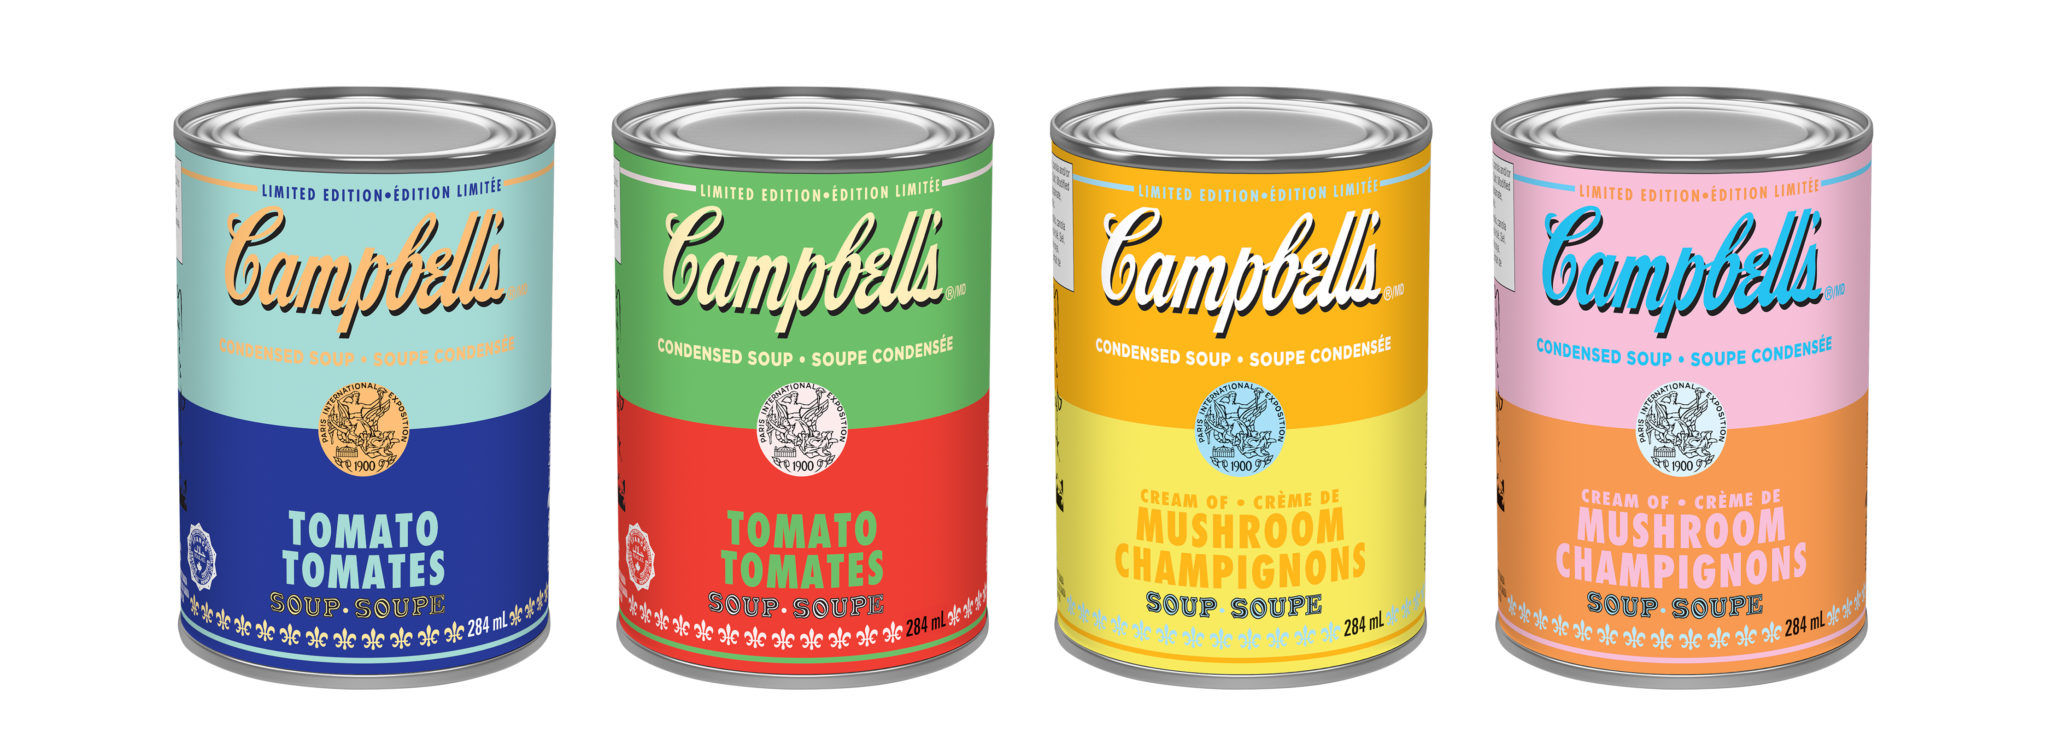
\includegraphics[width=15cm]{gfx/soupcans} \\  % Picture
            
\includegraphics[width=15cm]{gfx/EagleScience_Logo_on_white} \\  % Picture
            % Thesis subtitle
            % %\myDegree \\


            Begeleiding:\\ \bigskip
            EagleScience\\
            \myStagebegeleider \\
            \medskip
            Hogeschool van Amsterdam\\
            \myHvABegeleider \\ \bigskip \bigskip \bigskip


            \myTime % Time and version

            \vfill

        \end{center}
    \end{addmargin}

\end{titlepage}
 % Main title page

% Back of the title page

\thispagestyle{empty}

\hfill

\vfill

\noindent\myName: \textit{\myTitle,} \mySubtitle, %\myDegree, 
\textcopyright\ \myTime

% You may wish to do something with the back of the title page, such as including your supervisors, location or time frame of the work. Below is an example of doing so although you may want to tweak it to your liking.

%\bigskip

%\noindent\spacedlowsmallcaps{Supervisors}: \\
%\myProf \\
%\myOtherProf \\ 
%\mySupervisor

%\medskip \\

%\noindent\spacedlowsmallcaps{Location}: \\
%\myLocation

%\medskip \\

%\noindent\spacedlowsmallcaps{Time Frame}: \\
%\myTime
 % Back of the title page

%\cleardoublepage% Dedication

\thispagestyle{empty}
\refstepcounter{dummy}

\pdfbookmark[1]{Dedication}{Dedication} % Bookmark name visible in a PDF viewer

\vspace*{3cm}

\begin{center}
\emph{Ohana} means family. \\
Family means nobody gets left behind, or forgotten. \\ \medskip
--- Lilo \& Stitch    
\end{center}

\medskip

\begin{center}
Dedicated to the loving memory of Rudolf Miede. \\ \smallskip
1939\,--\,2005
\end{center} % Dedication page

%\cleardoublepage\include{FrontBackMatter/Foreword} % Uncomment and create a Foreword.tex to include a foreword

\cleardoublepage% Abstract

%\renewcommand{\abstractname}{Abstract} % Uncomment to change the name of the abstract

\pdfbookmark[1]{Samenvatting}{Samenvatting} % Bookmark name visible in a PDF viewer

\chapter{Samenvatting}\label{ch:samenvatting}

De in dit afstudeerverslag beschreven afstudeeropdracht is uitgevoerd in opdracht van Eaglescience, een bedrijf welke software op maat ontwikkeld voor een grote verscheidenheid aan klanten. Tijdens de ontwikkeling van software maakt Eaglescience gebruik van externe bibliotheken. Door het gebruik hiervan zouden er echter potentiele gevaren kunnen worden geintroduceerd in de software. Om deze gevaren inzichtelijk te maken, zodat hierop actie kan worden ondernomen, zou Eaglescience een geautomatiseerde analyse methode willen inzetten. In dit afstudeerverslag worden de onderzoeken beschreven die zijn uitgevoerd met als doel om een applicatie te ontwerpen die geautomatiseerd en periodiek de kwetsbaarheden van externe bibliotheken, ofwel 'software of unknown provencance' (SOUP) in kaart kan brengen.
Tijdens het onderzoek zijn de eisen aan deze applicatie vanuit de opdrachtgever in kaart gebracht, en is er onderzocht welke tooling en methodiek het beste aansluit bij de huidige werkwijze, Dev-stack en tooling van Eaglescience. Het onderzoek wees uit dat Eaglescience werkt met Scala en TypeScript, waarbij SBT en NPM als buildtools worden gebruikt. Door ontwikkeling in deze niche-taal is de beschikbare tooling voor SOUP analyses gelimiteerd. De resultaten van het onderzoek gaven aan dat de OWASP-dependency-check (voor NPM) en de sbt-dependency-check (voor SBT) het beste kunnen worden gebruikt. Na het uitvoeren van een reeks testen met deze tooling bleek deze inderdaad geschikt te zijn voor de specifieke situatie van Eaglescience en te voldoen aan de eisen van de opdrachtgever. Op basis van de informatie komende uit deze onderzoeken is een ontwerp ontwikkeld voor een applicatie, welke geautmatiseerd en op periodieke basis SOUP analyses uit zou kunnen voeren. De ontworpen applicatie voldoet aan de eisen gesteld door de opdrachtgever en zou daarom binnen de huidige Dev-stack kunnen worden geimplementeerd.





\vfill
 % Abstract page

%\cleardoublepage% Publications - a page listing research articles written using content in the thesis

\pdfbookmark[1]{Publications}{Publications} % Bookmark name visible in a PDF viewer

\chapter*{Publications} % Publications page text

Some ideas and figures have appeared previously in the following publications:\\

\noindent Put your publications from the thesis here. The packages \texttt{multibib} or \texttt{bibtopic} etc. can be used to handle multiple different bibliographies in your document.

%\begin{refsection}[ownpubs]
%    \small
%    \nocite{*} % is local to to the enclosing refsection
%    \printbibliography[heading=none]
%\end{refsection}

%\emph{Attention}: This requires a separate run of \texttt{bibtex} for your \texttt{refsection}, \eg, \texttt{ClassicThesis1-blx} for this file. You might also use \texttt{biber} as the backend for \texttt{biblatex}. See also \url{http://tex.stackexchange.com/questions/128196/problem-with-refsection}. % Publications from the thesis page

%\cleardoublepage% Acknowledgements

\pdfbookmark[1]{Acknowledgements}{Acknowledgements} % Bookmark name visible in a PDF viewer

\begin{flushright}{\slshape    
We have seen that computer programming is an art, \\ 
because it applies accumulated knowledge to the world, \\ 
because it requires skill and ingenuity, and especially \\
because it produces objects of beauty.} \\ \medskip
--- \defcitealias{knuth:1974}{Donald E. Knuth}\citetalias{knuth:1974} \citep{knuth:1974}
\end{flushright}

\bigskip

%----------------------------------------------------------------------------------------

\begingroup

\let\clearpage\relax
\let\cleardoublepage\relax
\let\cleardoublepage\relax

\chapter*{Acknowledgements}

\noindent Put your acknowledgements here.\\

\noindent Many thanks to everybody who already sent me a postcard!\\

\noindent Regarding the typography and other help, many thanks go to Marco Kuhlmann, Philipp Lehman, Lothar Schlesier, Jim Young, Lorenzo Pantieri and Enrico Gregorio\footnote{Members of GuIT (Gruppo Italiano Utilizzatori di \TeX\ e \LaTeX )}, J\"org Sommer, Joachim K\"ostler, Daniel Gottschlag, Denis Aydin, Paride Legovini, Steffen Prochnow, Nicolas Repp, Hinrich Harms, Roland Winkler, and the whole \LaTeX-community for support, ideas and some great software.

\bigskip

\noindent\emph{Regarding \mLyX}: The \mLyX\ port was initially done by
\emph{Nicholas Mariette} in March 2009 and continued by
\emph{Ivo Pletikosi\'c} in 2011. Thank you very much for your work and the contributions to the original style.

\endgroup % Acknowledgements page

\pagestyle{scrheadings} % Show chapter titles as headings

\cleardoublepage% Table of Contents - List of Tables/Figures/Listings and Acronyms

\refstepcounter{dummy}

\pdfbookmark[1]{\contentsname}{tableofcontents} % Bookmark name visible in a PDF viewer

\setcounter{tocdepth}{2} % Depth of sections to include in the table of contents - currently up to subsections

\setcounter{secnumdepth}{3} % Depth of sections to number in the text itself - currently up to subsubsections

\manualmark
\markboth{\spacedlowsmallcaps{\contentsname}}{\spacedlowsmallcaps{\contentsname}}
\tableofcontents
\automark[section]{chapter}
\renewcommand{\chaptermark}[1]{\markboth{\spacedlowsmallcaps{#1}}{\spacedlowsmallcaps{#1}}}
\renewcommand{\sectionmark}[1]{\markright{\thesection\enspace\spacedlowsmallcaps{#1}}}

\clearpage

\begingroup
\let\clearpage\relax
\let\cleardoublepage\relax
\let\cleardoublepage\relax

%----------------------------------------------------------------------------------------
%	List of Figures
%----------------------------------------------------------------------------------------

\refstepcounter{dummy}
%\addcontentsline{toc}{chapter}{\listfigurename} % Uncomment if you would like the list of figures to appear in the table of contents
\pdfbookmark[1]{\listfigurename}{lof} % Bookmark name visible in a PDF viewer

\listoffigures

\vspace{8ex}
\newpage

%----------------------------------------------------------------------------------------
%	List of Tables
%----------------------------------------------------------------------------------------

\refstepcounter{dummy}
%\addcontentsline{toc}{chapter}{\listtablename} % Uncomment if you would like the list of tables to appear in the table of contents
\pdfbookmark[1]{\listtablename}{lot} % Bookmark name visible in a PDF viewer

\listoftables

\vspace{8ex}
\newpage

%----------------------------------------------------------------------------------------
%	List of Listings
%----------------------------------------------------------------------------------------

\refstepcounter{dummy}
%\addcontentsline{toc}{chapter}{\lstlistlistingname} % Uncomment if you would like the list of listings to appear in the table of contents
\pdfbookmark[1]{\lstlistlistingname}{lol} % Bookmark name visible in a PDF viewer

\lstlistoflistings

\vspace{8ex}
\newpage

%----------------------------------------------------------------------------------------
%	Acronyms
%----------------------------------------------------------------------------------------

\refstepcounter{dummy}
%\addcontentsline{toc}{chapter}{Acronyms} % Uncomment if you would like the acronyms to appear in the table of contents
\pdfbookmark[1]{Acronyms}{acronyms} % Bookmark name visible in a PDF viewer

\markboth{\spacedlowsmallcaps{Acronyms}}{\spacedlowsmallcaps{Acronyms}}

\chapter*{Acroniemen}

\begin{acronym}[UML]
\acro{DRY}{Don't Repeat Yourself}
\acro{API}{Application Programming Interface}
\acro{UML}{Unified Modeling Language}
\end{acronym}

\endgroup
 % Contents, list of figures/tables/listings and acronyms

\cleardoublepage

\pagenumbering{arabic} % Arabic page numbering for thesis content (1, 2, 3, etc)
%\setcounter{page}{90} % Uncomment to manually start the page counter at an arbitrary value (for example if you wish to count the pre-content pages in the page count)

\cleardoublepage % Avoids problems with pdfbookmark

%----------------------------------------------------------------------------------------
%	THESIS CONTENT - CHAPTERS
%----------------------------------------------------------------------------------------


\part{Opdracht}\label{prt:opdracht}

% Chapter 1
\chapter{Eaglescience}\label{ch:Eaglescience} % Chapter title

Het hier beschreven onderzoek en het daarbij behorende ontwerp voor een applicatie is uitgevoerd en ontwikkeld in opdracht van het bedrijf Eaglescience. Dit bedrijf is gevestigd in Amsterdam Sloterdijk en houdt zich sinds 2009 bezig met het ontwikkelen van software. Hoewel het ontwikkelen van maatwerk software de kern activiteit is biedt het bedrijf ook een aantal andere diensten aan, zoals het bouwen van prototypes of het meedenken in een design sprint om bedrijven en startups een goede richting te geven voor het ontwikkelen van een project. Daarnaast biedt Eaglescience hosting aan voor de software die door hun is ontwikkeld, om zo garantie te kunnen bieden dat er alles aan wordt gedaan zodat de geleverde software veilig, kwalitatief goed en correct functioneert.

\section{Organisatie}\label{sec:organisatie}
Eaglescience BV bestaat uit drie divisies: Innovations, Software en Solutions (figuur~\ref{fig:Eaglescience organogram}). Er werken, op het moment van schrijven, $\pm$ 20 medewerkers waarvan 75\% verantwoordelijk is voor de ontwikkeling van software. De andere 25\% bekleed een support rol zoals project manager, finance manager, quality manager, automatisering etc.

\begin{figure}[bth]
\myfloatalign
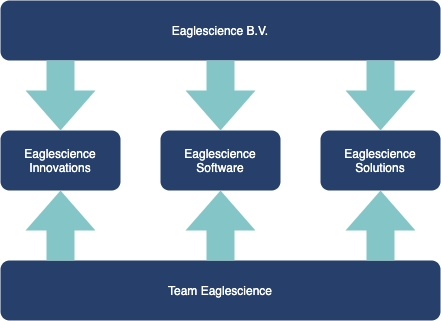
\includegraphics[width=9cm]{gfx/organogram}
\caption{Organogram Eaglescience}
\label{fig:Eaglescience organogram}
\end{figure}
De divisie Eaglescience Innovations zoekt naar nieuwe oplossingen op het gebied van softwareontwikkeling, welke door de divisie Eaglescience Software wordt geïmplementeerd. Eaglescience Solutions onderzoekt en adviseert over oplossingen voor gestelde problemen. Onder het dagelijks bestuur valt Team Eaglescience dat bestaat uit projectmanagers en ontwikkelaars. Deze zijn onderverdeeld in diverse scrum teams die ieder verantwoordelijk zijn voor een project. De ontwikkelaars worden parallel ingezet op meerdere projecten om kennisdeling te bevorderen.

\subsection{Missie}\label{subsec:missie}

De missie van Eaglescience is het bedienen van haar partners door een ontwerp, ontwikkeling en service te bieden op het gebied van op maat gemaakte IT-oplossingen. Hiervoor heeft Eaglescience goed opgeleide IT-professionals in dienst die zichzelf continue ontwikkelen op de “cutting edge” van IT-technologie. De hoofdcompetenties van de medewerkers zijn: innovatief, intelligent, klant georiënteerd, flexibel en ambitieus~\citep{Eaglescience:2020}.

\subsection{Visie}\label{subsec:visie}
Eaglescience streeft er als innovatief IT-bedrijf naar om software te ontwikkelen als een Business-to-Business dienst. Middels technische vaardigheden bouwen we veilige en hoogwaardige software die bijdraagt aan een betere wereld. Omdat we Agile werken, leveren we precies wat nodig is, niets meer en niets minder. Wij helpen onze klanten zoeken naar een langdurige betrokkenheid en samenwerking op basis van zowel vertrouwen als wederzijds respect.

Omdat elke vraag uniek is, ontwikkeld Eaglescience op maat gemaakte en innovatieve software.  We zijn van plan deel uit te maken van het hele proces van het formuleren van een idee tot het lanceren van het product en het waarborgen van de productie levenscyclus. Onze belangrijkste succesfactor zijn de mensen, die zich continu ontwikkelen door met de nieuwste technieken te werken op diverse projecten. Wij streven naar een optimale balans tussen werk en privé. Dit geeft onze medewerkers veel vrijheid, maar vereist zelfdiscipline en verantwoordelijkheid~\citep{Eaglescience:2020}.

\subsection{Strategie}\label{subsec:strategie}
Eaglescience levert de visie via vier strategische thema's:
\begin{itemize}
    \item Maatschappelijke verantwoordelijkheid
    \item Persoonlijke groei en werknemer tevredenheid
    \item Kwalitatief hoogstaande producten en diensten
    \item Financieël onafhankelijk en een sociaal verantwoorde groei
\end{itemize}
We streven er naar om veilige en hoogwaardige software diensten te leveren die waarde toevoegen aan onze samenleving. We streven naar een bedrijfscultuur waarin alle collega's hun talenten kunnen laten groeien. We hebben een ongecompliceerd werkethos: we richten ons op resultaten van hoge kwaliteit, maar met een gezonde balans tussen werk en privé en voldoende tijd voor leuke en sociale evenementen.
\newpage
Eaglescience verwacht van alle medewerkers dat zij hun handelen baseren op vier kwaliteitsprincipes:
\begin{itemize}
    \item Meld situaties die niet voldoen aan onze interne procedures
    \item Evalueer risico's wanneer grote veranderingen worden verwacht
    \item Help en daag elkaar uit
    \item Kennis behouden over conformiteit en kwaliteitsmanagement
\end{itemize}

\section{Werkwijze}\label{sec:werkwijze}
Zoals eerder gemeld werkt Eaglescience op projectbasis met ontwikkelaars in meerdere teams. Er wordt geprobeerd $"$full scrum$"$ te werken waarbij de requirements van de klant centraal staan. Als een project wordt aangenomen dan wordt deze in sprints in samenspraak met de klant ontwikkeld. De klant wordt nauw betrokken bij het verloop van de ontwikkeling door het geven van demo's aan het einde van iedere sprint. Hier wordt gemeten hoe de applicatie zich gedraagt met betrekking tot de requirements van de klant. Dit is ook het moment dat er feedback gegeven wordt en waar nodig gestuurd kan worden in het verdere verloop. Op het moment dat er een applicatie klaar is wordt de software al dan niet overgedragen aan de klant of doorgegeven aan support en hosting die verantwoordelijk zijn voor de daadwerkelijke hosting van de software.

\begin{figure}[bth]
\myfloatalign
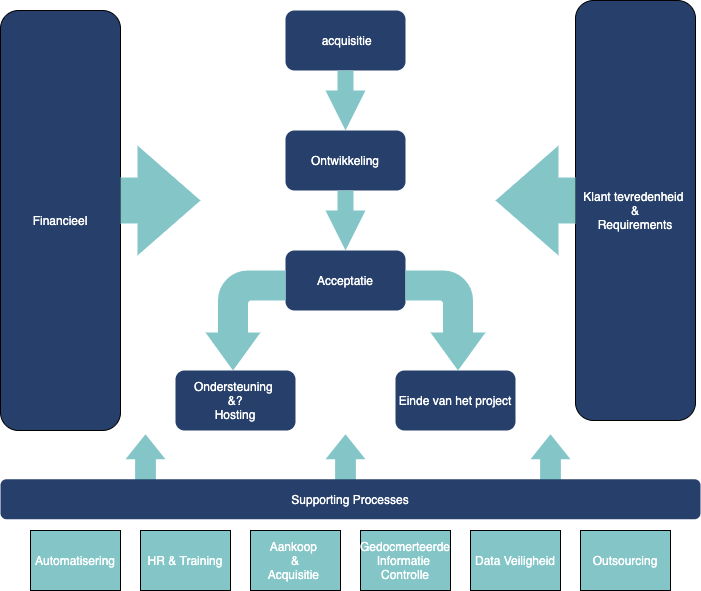
\includegraphics[width=12cm]{gfx/ProcessFlow}
\caption{Project Process}
\label{fig:Project Process}
\end{figure}

Naast het ontwikkelproces zijn er een aantal supporting processen die ervoor zorg dragen dat het bedrijf blijft draaien. Onder deze processen valt ook automatisering die voor ondersteuning zorgt van platformen waarop ontwikkeld en/of gehost wordt. Eaglescience ontwikkeld en genereert inkomsten op projectbasis. Alle processen die draaien moeten dus direct ingezet kunnen worden op projecten van klanten (figuur~\ref{fig:Project Process}). Als er een project voor intern gebruik wordt ondernomen moet er een duidelijk beeld zijn of er op termijn winst mee te behalen valt.

\section{Relevante en actuele ontwikkelingen binnen Eaglescience}\label{sec:relevante-en-actuele-ontwikkelingen-binnen-Eaglescience}

Eaglescience is aan het groeien, zowel in het aantal projecten als in het aantal medewerkers. Daarnaast worden de diensten die Eaglescience aanbied ook uitgebreid, en wordt het hosten van de ontwikkelde applicaties steeds vaker aangeboden. Door deze inzet ligt de verantwoordelijkheid niet alleen bij het leveren van een veilige en hoogwaardige software, maar ook bij het leveren van een veilige hosting service. Naast de groei van het bedrijf is ook de uitbreiding van diensten die aangeboden worden een reden om taken die geautomatiseerd kunnen worden dan ook te automatiseren.

Daarnaast heeft Eaglescience de afgelopen jaren een portfolio van verschillende klantproducten opgebouwd. Deze producten worden gehost, onderhouden en er wordt service en support geboden richting gebruikers. Eaglescience is momenteel dit onder de noemer Software Lifecycle Management aan het integreren in het kwaliteitssysteem door middel van beleid en het vastleggen in werkprocessen. Het in de grip en up-to-date houden van de live softwareproducten vraagt om een gerichte-, transparante- en traceerbare aanpak ten aanzien van alle gebruikte software-onderdelen (bibliotheken/ libraries) en onderliggende afhankelijkheden (dependencies).



 % Chapter 1
% Chapter 2

\chapter{Opdracht}\label{ch:opdracht} % Chapter title
Tegenwoordig zijn software-bibliotheken niet meer weg te denken uit het huidige software-ontwikkelproces. Bibliotheken geven ontwikkelaars de mogelijkheid code te hergebruiken in meerdere projecten, om zo efficiënter te kunnen ontwikkelen. Dit helpt op zijn beurt om de time-to-market te verkorten. Bibliotheken kunnen door bedrijven zelf geschreven worden, in het geval van Eaglescience is dit ArchES, of worden overgenomen van andere bedrijven/instellingen. ArchES is echter zelf ook afhankelijk van een aantal bibliotheken die niet ontwikkeld zijn door Eaglescience. Hierdoor kan niet worden voorkomen dat bibliotheken worden gebruikt waarvan de afkomst niet geheel kan worden herleid.

Deze (deels) onherleidbare bibliotheken vallen onder de noemer "Software of Unknown Provenance / Pedigree (SOUP)". Door het gebruik van dit soort bibliotheken kan er een aannemelijk risico ontstaan op het gebied van kwetsbaarheden. Om inzicht te verkrijgen in deze kwetsbaarheden en daarmee mogelijke veiligheidsissues dient een SOUP-analyse gedaan te worden. Binnen Eaglescience wordt het belang hiervan onderstreept en daarom wordt er gezocht naar een efficiënte en, waar mogelijk, geautomatiseerde manier voor het uitvoeren van een dergelijke analyse. Hierdoor kan de veiligheid van de ontwikkelde applicaties worden gewaarborgd zonder afbreuk te doen aan kwaliteit.

\section{Opdracht vanuit Eaglescience}\label{sec:opdracht-vanuit-Eaglescience}

Vanuit de CTO is de wens ontstaan om een systematisch opgebouwde methode te ontwikkelen waarbij er automatisch periodiek een SOUP-analyse gedaan wordt op bestaande en nieuwe projecten. Het beoogde resultaat is een module die wordt toegevoegd aan de al bestaande portal van Eaglescience waarbij project verantwoordelijken inzicht kunnen verkrijgen in de kwetsbaarheden die in een project aanwezig kunnen zijn door het gebruik van externe bibliotheken.

De aanleiding van deze opdracht is een gebrek aan inzicht in reeds draaiende software. In tegenstelling tot software waaraan nog ontwikkeld wordt, gaat er bij projecten waaraan niet actief wordt ontwikkeld het inzicht in gebruikte bibliotheken en hun versies verloren. Hierdoor is het onbekend welke kwetsbaarheden er mogelijk zijn in deze projecten.
\subsection{Eisen aan de opdracht}\label{subsec: eisen-aan-de-opdracht}
Vanuit Eaglescience worden er een aantal eisen gesteld waaraan het eindproduct moet voldoen. Als er aan deze eisen is voldaan is er voor Eaglescience een waardevol product ontwikkeld welke in gebruik kan worden genomen. Daarnaast zijn er een aantal opleveringseisen die gehaald dienen te worden om de kwaliteit te waarborgen. Ook is er aangegeven dat er bij voorkeur naar open source tooling dient gekeken te worden, daar er geen budget voor aanschaf van software voor handen is.
\newpage

\textbf{Functionele eisen}
\begin{itemize}
\item De module dient eenvoudig te kunnen worden gebruikt in de huidige Continuous Integration /Continuous Deployment (CI/CD) pipeline voor bestaande en nieuwe projecten
\item De module dient gebruik te maken van de bestaande huidige projectstructuur van de portal
\item De module dient ondersteuning te bieden aan meerdere omgevingen (OTAP)
\item De module dient te worden ontwikkeld in Angular en Play (Scala), zodat het in de bestaande portal module past
\item De module dient met een instelbaar interval de analyse uit te voeren
\item De module moet op project en omgeving niveau rapporteren over bekende kwetsbaarheden
\item De module dient kwetsbaarheden op minimaal drie niveau’s in te schalen (kritisch, gemiddeld en laag)
%\item De module dient ondersteuning te bieden voor het instellen van quality gates ten aanzien van de melding die het vind van ieder niveau, per project, per omgeving
\end{itemize}
\textbf{Kwaliteitseisen}
\begin{itemize}
\item De module dient te voldoen aan de geldende kwaliteitsnormen binnen Eaglescience, minimaal meetbaar door:
	\begin{itemize}
	\item Test coverage > 70\%
	\item Onderdeel van de bestaande CI/CD voor de Eaglescience Portal
	\end{itemize}
\item De geschreven code dient gereviewd te worden door een Eaglescience ontwikkelaar
\item De module dient gescheiden componenten te bevatten: Frontend, Backend, API
\item Voor de API dient gebruik te worden gemaakt van swagger
\item De module dient goed gedocumenteerd te zijn middels 'in code comments'
\end{itemize}

\subsection{Deliverables vereiste resultaten}\label{subsec:deliverables-vereiste-resultaten}
Vanuit de CTO worden er naast de functionele eisen ook eisen gesteld aan de oplevering:
\begin{itemize}
\item Geïntegreerde en aantoonbaar werkende module
\item De code van de module is gepubliceerd in Eaglescience GitLab
\item Aanwezigheid van een handleiding over hoe de module gebruikt dient te worden
\item Eventuele aanvullende deliverables vanuit de HvA
\end{itemize}

\section{Gewenst neveneffect}\label{sec:gewenst-neveneffect}
Naast dat de nieuwe module inzicht moet geven in de kwetsbaarheden van bibliotheken van derden zal deze ook bewustzijn creëren in risico's van het gebruik hiervan. Voordat er zal worden overgegaan tot het gebruik van een bibliotheek dienen de volgende vragen te worden beantwoord:
\begin{itemize}
	\item Is deze bibliotheek echt nodig?
	\item Zo ja, welke invloed heeft dat op de veiligheid van de applicatie?
	\item Kan deze functionaliteit ook op een andere eenvoudige manier worden bewerkstelligd?
	\item Is er een andere bibliotheek die dezelfde functionaliteiten biedt?

\end{itemize}


\section{Opdracht fasen}\label{sec:opdracht-fasen}
Om de hierboven beschreven opdracht zo goed als mogelijk uit te voeren dient er eerst een onderzoek gedaan te worden naar begrippen binnen het domein SOUP, de ontwikkelomgeving van Eaglescience en daarnaast naar mogelijkheden om bibliotheken te screenen en te testen op kwetsbaarheden. Na de onderzoeksfase moet er een module ontwikkeld worden die deze mogelijkheid implementeert met inachtneming van de hierboven genoemde eisen.

\subsection{Fase 1: Onderzoek} \label{subsec:fase-1:-onderzoek}
Als eerste dient er onderzoek gedaan te worden naar de huidige situatie binnen Eaglescience waarbij er gekeken wordt naar de huidige dev-stack, de tooling, de werkwijze, als ook de huidige manier van uitrollen van applicaties. Daarna dient er een begrippen / literatuur onderzoek gedaan te worden binnen het domein SOUP om een goede kennis te vergaren over het domein om een basis te kunnen leggen voor een te implementeren module. Daarnaast dient er onderzoek gedaan te worden om te zien of er bibliotheken en resources zijn waar informatie over SOUP-bibliotheken te vinden is, en aan welke eisen deze bibliotheken moeten voldoen om kwetsbaar te worden. Hier lettende op de eisen vanuit Eaglescience en de mogelijkheden die deze analyse bibliotheken bieden. Deze fase wordt beschreven in het deel~\ref{prt:Onderzoek} van dit document.

\subsection{Fase 2: Oplevering SOUP analyse module}\label{subsec:fase-2:-oplevering-soup-analyse-module}
De uit het onderzoek behaalde resultaten aangaande beschikbare resources om een SOUP-analyse uit te voeren vormen een leidraad voor de implementatie van de module. Deze module moet voldoen aan de eisen die gesteld zijn. Het ontwerp wordt beschreven in deel~\ref{prt:ontwerp}

\cleardoublepage % Empty page before the start of the next part

%------------------------------------------------

\part{Onderzoek}\label{prt:Onderzoek} % Second part of the thesis
\chapter{Onderzoeksplan}\label{ch:onderzoekPlan}

In het vorige hoofdstuk is de opdracht voor dit onderzoek beschreven. In dit hoofdstuk wordt uitgewijd over hoe deze opdracht en het daarbij behorende onderzoek zal worden uitgevoerd en welke bronnen er hiervoor gebruikt worden. Het resultaat is een onderzoeksplan voor een onderzoek naar analyses op kwetsbaarheden in externe bibliotheken (SOUP) binnen Eaglescience.


\section{Aanleiding}\label{sec:OP_aanleiding}
Eaglescience heeft de ambitie om te groeien in zowel het aantal projecten dat het aanneemt als in het aantal medewerkers. Daarnaast is het bezig met het integreren van het software lifecycle management paradigma in het kwaliteitssysteem om zo een gerichte-, transparante en traceerbare aanpak te hebben aangaande de kwaliteit en daarmee de veiligheid van de te leveren software. Er wordt gezocht naar manieren om taken die veel voorkomen en bijdragen aan de kwaliteit te automatiseren om op die manier een traceerbare en transparante aanpak te verkrijgen. Op dit moment mist voornamelijk inzicht in de kwetsbaarheden van projecten waarvan de ontwikkeling is afgerond, maar die wel door Eaglescience worden gehost en daardoor onder haar verantwoordelijkheid vallen.


\section{Probleemanalyse}\label{sec:probleemanalyse}
Eaglescience doet veel om veilige applicaties te leveren aan haar klanten. Tijdens het ontwikkelproces wordt er door de ontwikkelaars continue afgewogen welke maatregelen, in architectuur en/of code, moeten worden genomen om applicaties veilig op te kunnen leveren. Deze afwegingen zijn onderdeel van het ontwerpproces en worden door de klant gezien als declarabele uren en zij zijn dan ook bereid voor deze werkzaamheden te betalen. Op het moment dat een project 'klaar' is en over gaat van ontwikkeling naar hosting wordt er onderhoud gedaan volgens afspraken in de SLA. In diezelfde SLA wordt niet altijd ruimte opgenomen voor het testen van de applicatie op kwetsbaarheden middels SOUP-analyses. Vaak komt dit doordat de klant er geen budget voor heeft, of het niet belangrijk vindt. Gezien Eaglescience alleen een advies kan uitbrengen over support en de klant de eindbeslissing neemt worden SOUP-analyses vaak niet of niet tijdig uitgevoerd. Omdat Eaglescience wel "zo veel mogelijk" wil garanderen dat de software die gehost wordt veilig is, dient de applicatie in hosting periodiek geanalyseerd te worden op kwetsbaarheden. Op dit moment is dit een tijdrovend handmatig process waarmee een teamlid ongeveer 8 tot 12 uur bezig is. Voor iedere dependency moet er namelijk bekeken worden of er mogelijke kwetsbaarheden bestaan, of dan al niet geupdate moeten worden. Door de groei die Eaglescience binnenkort wil maken bestaat de wens om bovenstaand proces te automatiseren.

Er moet dus een methode worden ontwikkeld die het mogelijk maakt om geautomatiseerd en periodiek een SOUP-analyse te doen op dependencies binnen een project. De SOUP-analyses moeten inzichtelijk maken of en zo ja, welke, kwetsbaarheden zijn gevonden in deze bibliotheken. De methode moet voor alle platformen (Docker, programmeertalen, databases etc.) dezelfde resultaten geven, en compatibel zijn met de huidige infrastructuur van Eaglescience.

Door de analyses te automatiseren wordt beoogd dat er minder tijd zal hoeven te worden besteed aan de analyse. Deze tijd kan dan worden ingezet door de ontwikkelaar aan taken die declarabel zijn en voor beide partijen winstgevend zijn.


\section{Probleem stelling, onderzoeksvraag en doelstellingen}\label{sec:probleem-stelling-onderzoeksvraag-en-doelstellingen}
Samengevat luidt het probleem: Het handmatig uitvoeren van SOUP-analyses kost manuren die niet declarabel zijn. Om deze reden is de wens dat er een geautomatiseerde oplossing komt die periodiek de projecten, die in ontwikkeling zijn en/of door Eaglescience gehost worden, analyseert op kwetsbaarheden in gebruikte externe bibliotheken. Door deze automatische oplossing te gebruiken wordt beoogd dat de (niet declarabele) uren die normaal gebruikt worden voor het analyseren van projecten in plaats daarvan gebruikt kunnen worden voor andere wel declarabele uren. Hierdoor zou de efficiëntie binnen Eaglescience kunnen worden verhoogd.

Voor het onderzoek naar het hierboven genoemde probleem is de volgende centrale onderzoeksvraag opgesteld: "Hoe kan Eaglescience middels een geautomatiseerde methode inzicht krijgen in potentiële kwetsbaarheden van gebruikte bibliotheken binnen projecten, waarbij rekening gehouden wordt met de huidige manier van werken?"

De opdracht heeft de volgende doelstelling:
Het doel van dit onderzoek is het ontwikkelen van een methode om SOUP-analyses uit te voeren binnen de dev-stack van Eaglescience. Hierbij moet rekening gehouden worden met de in de opdracht gegeven criteria. Aan het einde van het onderzoek moet een methode worden gepresenteerd die vervolgens bewezen kan worden middels een implementatie van een analyse op de twee meest gebruikte technologieën binnen Eaglescience, Scala en TypeScript.


\section{Stakeholderanalyse}\label{sec:stakeholdersanalyse}
Om inzicht te verkrijgen in het draagvlak voor dit onderzoek dient er een stakeholders analyse gedaan te worden. Op deze manier moet het duidelijk worden wie de stakeholders zijn en welke belangen zij hebben bij het doen van een onderzoek naar een geautomatiseerde SOUP-analyse en de resultaten hiervan.

\subsection{Dagelijks bestuur (intern)}\label{subsec:dagelijks-bestuur-(intern)1}
Het dagelijks bestuur ziet vooral voordelen in het op een overzichtelijke manier verkrijgen van inzichten in kwetsbaarheden. Zij beogen dat ze hierdoor beter kunnen aansturen in het gebruik van bibliotheken en/of andere technologieën. Ondanks dat de ontwikkeling van de beoogde nieuwe module vooral geld zal kosten, is de huidige manier van werken ook niet kosten-effectief. Daarnaast voorziet de CTO dat de nieuwe module tijdswinst zal opleveren waardoor de time-to-market voor andere projecten hoger kan komen te liggen en er dus op langere termijn meer omzet gegenereerd kan worden.

\subsection{Projectmanagers (intern)}\label{subsec:projectmanagers-(intern)1}
Projectmanagers krijgen op dit moment een update over de staat van kwetsbaarheden na afronding van een analyse, welke vaak na een deploy plaatsvindt of op verzoek. De nieuwe module zal echter de mogelijkheid bieden om up-to-date informatie on-demand te verkrijgen.
De tijdsinvestering die nodig is van ontwikkelaars voor de ontwikkeling van de module weegt volgens hen op tegen de voordelen die de module in de toekomst kan brengen.

\subsection{Ontwikkelteam (intern)}\label{subsec:ontwikkelteam-(intern)1}
Het handmatig testen van kwetsbaarheden werd tot op vandaag gedaan door het ontwikkelteam. Dit is een tijdrovende taak, welke ten koste gaat van de ontwikkeling van software voor klanten. Het ontwikkelteam heeft daarom direct baat bij de ontwikkeling van de beoogde module en wil daarom graag hieraan meedenken en meewerken.

\subsection{Klant (extern)}\label{subsec:klant-(extern)1}
De enige externe stakeholder is de klant, welke ook een passieve stakeholder is, gezien zij niet direct betrokken zijn bij de ontwikkeling van de module, maar wel baat hebben bij de uitkomst hiervan, namelijk in de vorm van veiligere en betrouwbaardere software tegen potentieel lagere kosten.

\begin{figure}
    \myfloatalign
    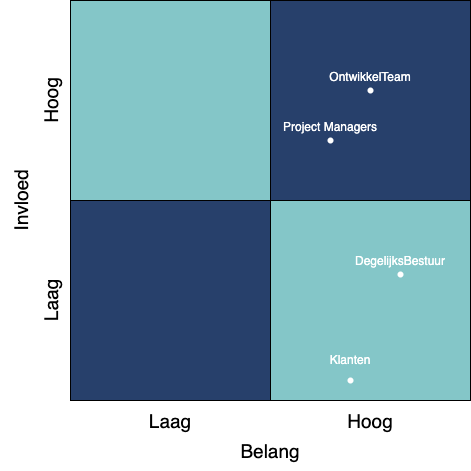
\includegraphics[width=10cm]{gfx/stakeholderanalyse}
    \caption{StakeHolders Analyse}
    \label{fig:StakeholderAnalyse1}
\end{figure}
Zoals te zien is in figuur~\ref{fig:StakeholderAnalyse1} is hebben alle stakeholders veel baat bij een nieuwe module voor de analyse van kwetsbaarheden. De invloed hierop is het hoogst bij het ontwikkelteam en de projectmanagers. De lage invloed van de klant zorgt ervoor dat voor het ontwerp alleen de requirements vanuit Eaglescience worden opgenomen.

\section{Theoretisch kader}\label{sec:theoretisch-kader}
Het theoretisch kader waarmee wordt gewerkt bestaat uit twee delen. Het eerste deel omvat theorie over externe bibliotheken. Het richt zich op het gebruik hiervan en de potentiële gevaren en methoden om deze bibliotheken te analyseren. De geselecteerde bronnen zijn:
\begin{itemize}
    \item \textbf{OWASP top 10}
    De OWASP Top-10 is als uitgangspunt gekozen omdat de inhoud van dit document binnen Eaglescience geldt als aandachtspunt voor het ontwikkelen van veilige software. De basis voor dit onderzoek wordt beschreven in punt "A06:2021-Vulnerable and Outdated Components". Hier wordt beschreven welke gevaren er potentieel dreigen als op dit punt niets gedaan wordt~\citep{OWASP:2021}.
    \item \textbf{OWASP dependency-check} Pagina over het project binnen de OWASP voor het analyseren van componenten in applicaties~\citep{OWASP:2017}.
    \item \textbf{Justifying the use of software of uncertain pedigree (SOUP) in safety-related applications} Hoewel dit document verouderd lijkt staat er wel degelijk interessante informatie over waarom je SOUP zou gebruiken en hoe je de risico's kan verminderen~\citep{Bischop:2001} .
    \item \textbf{Backstabber’s Knife Collection: A Review of Open Source Software Supply Chain Attacks}Dit artikel bevat informatie over een mogelijke vorm van aanvallen die middels SOUP uitgevoerd zouden kunnen worden. Daarnaast geeft het artikel inzicht in hoe de onderzoekers packages voor NPM, Python, en Ruby hebben onderzocht op kwetsbaarheden~\citep{Ohm:2020}.
\end{itemize}
Het tweede deel omvat de werkwijze van Eaglescience en de door hun gebruikte technologieën. De geselecteerde documenten vormen de basis informatie over de werkwijze van Eaglescience en zal als input worden gebruikt bij het ontwerp van de analyse die aansluitend aan het onderzoek zal plaatsvinden. De volgende bronnen zullen bij het onderzoek worden gebruikt:
\begin{itemize}
    \item \textbf{151030 F04B Proces Flow Chart ES\_V1.0\_TN.pdf} Een document dat de workflow beschrijft die binnen Eaglescience gehanteerd wordt~\citep{Eaglescience:2015}.
    \item \textbf{200121\_Policy Manual\_ES\_V6 signed.pdf} ISO-handboek waarin de bedrijfsvoering binnen Eaglescience wordt beschreven~\citep{Eaglescience:2020}.
\end{itemize}

\section{Conceptueel model}\label{sec:conceptueel-model}
Om de relevantie en relatie van de verschillende onderzoeken te waarborgen is een conceptueel model opgesteld(figuur~\ref{fig:ConceptueelModel}).
\begin{figure}
    \centering
    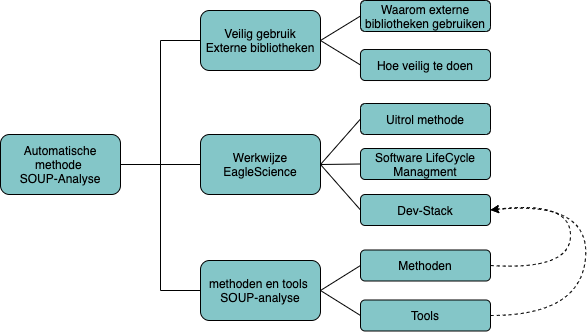
\includegraphics[width=12cm]{gfx/Conceptueel Model}
    \caption{Conceptueel Model}
    \label{fig:ConceptueelModel}
\end{figure}
Dit model maakt de samenhang van de verschillende begrippen inzichtelijk. Het kernbegrip is "Automatische methode SOUP-analyse" welke dit onderzoek uiteindelijk moet opleveren. Om hiertoe te komen zijn er drie begrippen die ieders een eigen domein binnen de probleemstelling belichten. In het theoretisch deel "Veilig gebruik externe bibliotheken"  wordt onderzocht waarom er bibliotheken van buitenaf worden gebruikt en wat de potentiële gevaren zijn die dit met zich meebrengt, en eventuele remedies hiervoor. Daarna zal "Werkwijze Eaglescience"  de manier van werken binnen Eaglescience belichten als ook de manier van uitrollen en de algehele dev-stack die Eaglescience gebruikt. Het begrip "Methoden en tools SOUP-analyse" zal ingaan op de beschikbare tools die gebruikt kunnen worden om een analyse te doen. Met deze tools wordt een methode onderzocht die SOUP-analyses mogelijk maakt binnen de dev-stack van Eaglescience. Samen zal dit onderzoek leiden tot een theoretische methode die als input kan gelden voor het ontwerp voor de nieuwe module die in de opdracht staat beschreven.

\section{Onderzoeksontwerp}\label{sec:OP_onderzoeksontwerp}
Aan de hand van de hierboven beschreven doelstellingen, theoretisch kader en conceptueel model is het volgende onderzoeksontwerp opgesteld.

\subsection{Onderzoeksvraag}\label{subsec:onderzoeksvraag-en-deelvragen}
Op basis van de probleemanalyse luidt de onderzoeksvraag als volgt: "Hoe kan Eaglescience middels een geautomatiseerde methode inzicht krijgen in potentiële kwetsbaarheden van gebruikte bibliotheken binnen projecten waarbij rekening gehouden wordt met de huidige manier van werken?". Door het ontleden van deze onderzoeksvraag ontstaan er twee delen waarnaar onderzoek gedaan moet worden. Het eerste deel is het gebruik en gevaar van externe bibliotheken, welke leidt tot de volgende onderzoeksvraag: "Wat is het effect van het gebruik van externe bibliotheken bij het ontwikkelen van software, welke gevaren brengt dit met zich mee en wat kan er gedaan worden om deze gevaren te minimaliseren?". Vervolgens kan deze kennis worden benut in het tweede deel, wat de praktische kant belicht, gericht op de methode en tooling voor SOUP-analyses. Dit tweede deel omvat methodes om geautomatiseerd SOUP-analyses te doen op projecten binnen Eaglescience. De onderzoeksvraag luidt als volgt: "Welke SCA tooling is compatibel met de omgeving van Eaglescience en welke methode kan worden toegepast om deze tooling te gebruiken voor het automatisch analyseren van externe dependencies?"

Deze delen zullen ieders in een deelonderzoek worden behandeld, waarvan de uitkomsten elkaar zullen aanvullen en samen tot een eind eindresultaat leiden.
\begin{figure}
    \myfloatalign
    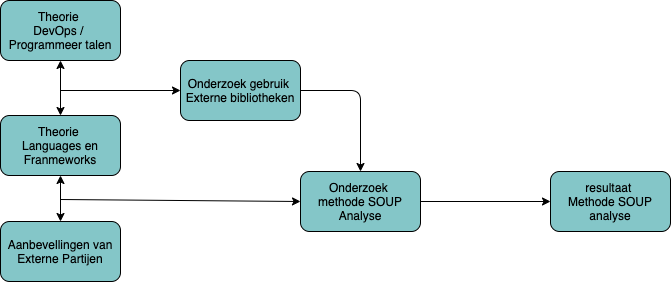
\includegraphics[width=12cm]{gfx/Onderzoekmodel}
    \caption{Onderzoeksmodel}
    \label{fig:OnderzoeksModel}
\end{figure}

In figuur\ref{fig:OnderzoeksModel} is te zien hoe de twee onderzoeken met elkaar in relatie staan ten opzichte van het beoogde eindresultaat. Het onderzoek over het gebruik van externe bibliotheken zal leiden tot concrete inzichten die vervolgens gebruikt kunnen worden als kennis in het onderzoek naar een methode voor een SOUP-analyse. Dit zal uiteindelijk een methode opleveren die gebruikt kan worden voor de implementatie van de module die aan de opdracht voldoet.

\subsection{Scope}\label{subsec:scope}
Het domein softwareveiligheid is op het moment van schrijven een 'hot-topic', en zeer breed. Om deze reden is er gekozen om dit onderzoek te beperken tot het veiliger maken van software middels het analyseren en beschikbaar stellen van informatie over externe bibliotheken. Daarnaast zullen alleen de technologieën die compatibel zijn met de werkwijze van Eaglescience mee worden genomen. Daarnaast is de opdracht zoals deze is gegeven door de CTO van Eaglescience de leidraad voor de scope van het onderzoek.

\subsection{Onderzoek strategie}\label{subsec:onderzoek-strategie}
Zoals hierboven is aangegeven zullen er een tweetal onderzoeken worden uitgevoerd. De conclusie van het eerste onderzoek zal dienen als input voor het tweede onderzoek.

%\newpage %TODO: quickfix om volgorde lijkheid te veranderen voor figuren...


\subsubsection{Onderzoek 1: gebruik externe bibliotheken, het gevaar en hoe veiliger te maken}
Het \textbf{doel} van dit onderzoek is om inzicht te krijgen in wat een SOUP-analyse is en hoe relevant het is om deze uit te voeren. Daarnaast wordt er gekeken wat de SOUP-analyse toevoegt aan de veiligheid van de software die Eaglescience levert en hoe Eaglescience mogelijk kan voorkomen dat er kwetsbaarheden in de uitgerolde software terecht komen.
De \textbf{scope} van dit onderzoek is dat er gekeken wordt naar het gebruik van externe bibliotheken en de toegevoegde waarde hiervan. Daarnaast wordt er gekeken wat er gedaan kan worden om het gebruik van externe bibliotheken veiliger te maken.
De \textbf{onderzoeksvraag} luid: "Wat is het effect van het gebruik van externe bibliotheken bij het ontwikkelen van software, welke gevaren brengt dit met zich mee en wat kan er gedaan worden om deze gevaren te minimaliseren?".
De gebruikte \textbf{methodes} zullen deskresearch zijn aangevuld met conferenties, waarbij \textbf{bronnen} zoals artikelen en rapportages van instanties en bedrijven die zich bezighouden met de veiligheid van software zullen worden opgenomen met als focus het gebruik van externe bibliotheken. Software veiligheid is een 'hot-topic' en er worden jaarlijks veel conferenties gehouden over dit onderwerp. Door de huidige wereld situatie is het mogelijk om veel van deze conferenties  ''on-demand'' terug te kijken wat op zijn beurt ook weer tot andere inzichten kan leiden. In figuur~\ref{fig:OnderzoeksModelNoodZaakSOUP} is te zien hoe het onderzoek is opgebouwd.
\begin{figure}[htbp]
    \myfloatalign
    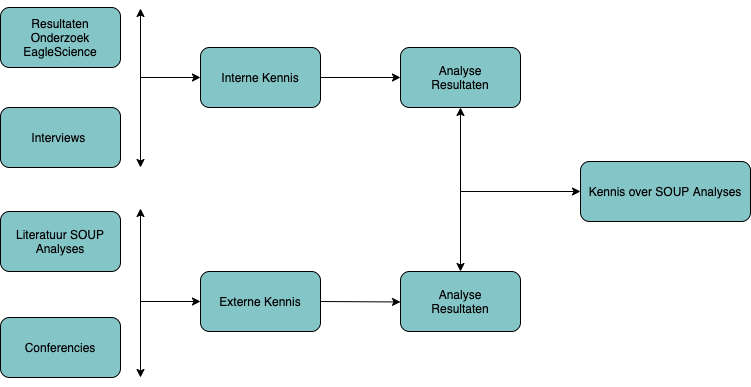
\includegraphics[width=12cm]{gfx/OnderzoeksmodelSOUP}
    \caption{Onderzoeksmodel gevaren van SOUP}
    \label{fig:OnderzoeksModelNoodZaakSOUP}
\end{figure}



\subsubsection{Onderzoek 2: tools en methodes voor SOUP-analyses op de Eaglescience dev-stack}
Het \textbf{doel} van dit onderzoek is om een methode te vinden die het mogelijk maakt om een SOUP-analyse te doen binnen de huidige dev-stack van Eaglescience. Hiervoor zullen er geschikte SCA (Software Composition Analysis) tools gevonden moeten worden. Binnen de \textbf{scope} van het onderzoek zal daarom alleen gekeken worden naar SCA tooling die analyses doet voor componenten binnen de dev-stack van Eaglescience. De \textbf{onderzoeksvraag} luidt: "Welke SCA tooling is compatibel met de omgeving van Eaglescience en welke methode kan worden toegepast om deze tooling te gebruiken voor het automatisch analyseren van externe dependencies?". De \textbf{methode} die gebruikt wordt is deskresearch. Daarnaast zullen er interviews gehouden worden met collega's om inzicht te krijgen in de huidige stand van zaken op het gebied van gebruik van externe bibliotheken en hoe er in de huidige situatie voor wordt gezorgd dat er geen kwetsbaarheden worden geïntroduceerd door het gebruik hiervan. Als er een selectie is gemaakt voor een tool dient deze in een kleine testopstelling getest te worden om vervolgens te kijken of deze kan worden geïmplementeerd in de bestaande uitrol methode. De \textbf{bronnen} die gebruikt zullen worden zijn informatie bronnen van leveranciers van dergelijke tooling. Ook zal er in interne documentatie worden gekeken hoe de huidige processen draaien waarin wordt beoogd om de SOUP-analyse uit te voeren. Daarnaast zullen de bevindingen middels een review worden geverifieerd op bruikbaarheid bij de opdrachtgever. Het onderzoeksmodel voor dit onderzoek is te vinden in figuur~\ref{fig:OnderzoeksModelSOUPmethode}.

\begin{figure}[htbp]
    \myfloatalign
    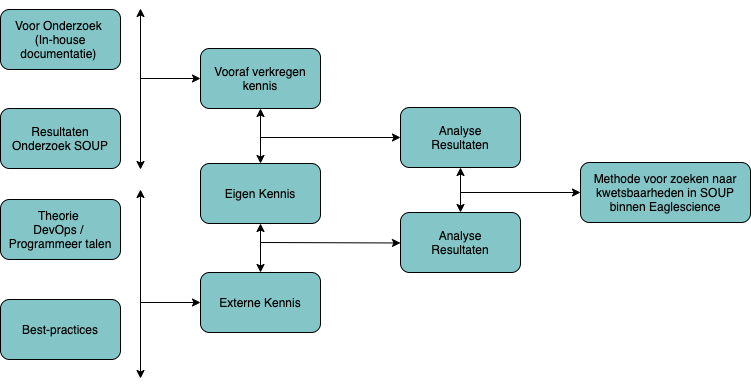
\includegraphics[width=12cm]{gfx/OnderzoeksModelSOUPMethode}
    \caption{Onderzoeksmodel SOUP-analyse module}
    \label{fig:OnderzoeksModelSOUPmethode}
\end{figure}

\section{Planning}\label{sec:planning}
Om tijdig tot resultaten te komen is de volgende planning opgesteld.

\subsection{Requirements analyse \textbf{september 2021}}\label{subsec:requirements-analyse}
Na het ontvangen van de opdracht dient er onderzocht te worden of er naast de eisen die door de CTO in de opdracht zijn gezet nog andere eisen zijn binnen Eaglescience. Hiervoor zal er onderzocht worden welke betrokkenen er zijn en welke belangen en wensen zij hebben. Na het houden van interviews zullen alle wensen tegen elkaar worden afgewogen. Dit zal leiden tot een document waarin alle belangrijke requirements worden geprioriteerd volgens de MoSCoW\-methode.

\textbf{Methode:} Intake gesprek met opdrachtgever, interviews met betrokkenen, enquete voor ontwikkelaars.

\textbf{Resultaat:} Applicatie requirements document.

\subsection{Vooronderzoek \textbf{september 2021 - oktober 2021 }}\label{subsec:onderzoek}
Om de requirements om te kunnen zetten naar een ontwerp zal er onderzoek gedaan worden naar de huidige manier van ontwikkelen en compileren van de software. Een onderzoek naar begrippen binnen het domein SOUP is een voorwaarde om vervolgens onderzoek te kunnen doen naar methodes om analyses te kunnen doen op software die Eaglescience maakt ten opzichte van SOUP. De resultaten van het vooronderzoek zullen worden gebruikt als input.
Om meer kennis en verdieping te krijgen in de materie rondom de nieuwe module zullen er een aantal onderzoeken worden uitgevoerd.


Er is onderzoek nodig naar de volgende onderwerpen:
\begin{itemize}
    \item \textbf{Externe bibliotheken gebruik en het gevaar}: Onderzoek naar waarom er externe bibliotheken worden gebruikt en het gevaar hiervan en hoe deze kunnen worden ondervangen.
    \item \textbf{SOUP Analyse binnen Eaglescience}: Dit onderzoek zal de tooling en methode in kaart brengen voor het uitvoeren van SOUP\-analyses binnen Eaglescience.
\end{itemize}

\textbf{Methode:} Bureau onderzoek, interviews met specialisten, deelnemen aan en/of terugkijken van conferenties, Sandbox testen met gevonden tooling.

\textbf{Resultaat:} Inzicht in het begrip SOUP en software veiligheid als ook een idee voor een mogelijke implementatie van de oplossing die voor Eaglescience de beste is zonder veel impact op de huidige manier van werken te hebben.

\subsection{Initieel ontwerp \textbf{oktober 2021 - november 2021 }}\label{subsec:initieel-ontwerp}
Er zal een ontwerp worden gemaakt waarin vast gelegd is welke requirements er beslist in de module moeten zitten en de uitwerking van deze. Evenals een ontwerp van de architectuur en het datamodel. Naast de module zal er ook een ontwerp gemaakt worden voor een ontwikkel/test omgeving om de module continue te kunnen testen zonder dat dit de huidige buildstraat beïnvloed. Dit laatste is van belang om zo min mogelijk storingen te veroorzaken in de dagelijkse gang van zaken bij al lopende projecten. Het eerste ontwerp zal als leidraad dienen voor de implementatie waarin afgeweken kan worden als dit nodig blijkt tijdens de implementatie sprints.

\textbf{Methode:} Overleggen met ontwikkelaars, huidige omgeving onderzoeken op mogelijkheden en architectuur.
\textbf{Resultaat:} Eerste ontwerp in de vorm van een datamodel, blokdiagram van architectuur voor de oplossing, als ook een sequentiediagram om van analyse tot rapportage te komen.

\subsection{Implementatie en Testen \textbf{november 2021 - januari 2022 }}\label{subsec:implementatie-en-testen}
Om te kunnen beginnen aan de implementatie is er een ontwikkel/ test omgeving nodig die het mogelijk maakt om zonder invloed op de dagelijkse werkzaamheden van Eaglescience een module te kunnen ontwikkelen. Deze zal eerst worden opgezet. Als test projecten zullen snapshots worden gebruikt van de daadwerkelijke projecten dit om een zo accuraat mogelijke test omgeving te hebben. Zoals in de opdracht beschreven dient de nieuwe module een onderdeel te zijn van de bestaande portal. Er zal dan ook direct samen worden gewerkt met het team die daar op het moment mee aan het ontwikkelen is. Tijdens de implementatie zal er ook worden gedocumenteerd wordt hoe de module werkt en welke procedures hier in worden gevolgd. Dit document biedt ontwikkelaars de mogelijkheid om dit door te nemen als on-boarding en referentie.

\textbf{Methode:} Agile scrum sprints met iedere 2 weken een oplevermoment en demo als ook een reflectie op de sprint.
\textbf{Resultaat:} Werkende en geteste applicatie die klaar is om uitgerold te worden.

\subsection{Uitrollen en documentatie \textbf{januari 2022 - februari 2022 }}\label{subsec:uitrollen-en-documentatie}
Nadat de implementatie van de meest kritische requirements is afgerond zal er worden begonnen met het uitrollen van de module en het testen door een geselecteerde groep gebruikers. De feedback wordt bekeken en meegenomen in de evaluatie. Mocht het nodig zijn dan zal er acuut actie worden ondernomen om deze wijzigingen aan te passen. Mochten er wensen zijn die kunnen wachten dan zal er worden overwogen om deze mee te nemen in de volgende iteratie van het project. Daarnaast zal ook de documentatie verder worden afgerond.
\textbf{Methode:} Interviews met stakeholders met een analyse over de nieuwe requirements.

\textbf{Resultaat:} Uitgerolde en gedocumenteerde applicatie.


\part{Old stuff}\label{prt:OldStuff}
% Chapter 1

\chapter{Introduction} % Chapter title

\label{ch:introduction} % For referencing the chapter elsewhere, use \autoref{ch:introduction} 

%----------------------------------------------------------------------------------------

This template for \LaTeX\ has two goals:
\begin{enumerate}
\item Provide students with an easy-to-use template for their Master's or PhD thesis (though it might also be used by other types of authors for reports, books, etc.).
\item Provide a classic, high-quality typographic style that is inspired by \citeauthor{bringhurst:2002}'s ``\emph{The Elements of Typographic Style}'' \citep{bringhurst:2002}.
\marginpar{\myTitle \myVersion}
\end{enumerate}

The bundle is configured to run with a \emph{full} MiK\TeX\ or \TeX Live installation right away and, therefore, it uses only freely available fonts.

People interested only in the nice style and not the whole bundle can now use the style stand-alone via the file \texttt{classicthesis.sty}. This works now also with ``plain'' \LaTeX.

As of version 3.0, \texttt{classicthesis} can also be easily used with \mLyX\footnote{\url{http://www.lyx.org}} thanks to Nicholas Mariette and Ivo Pletikosi\'c. The \mLyX\ version of this manual will contain more information on the details.

This should enable anyone with a basic knowledge of \LaTeXe\ or \mLyX\ to produce beautiful documents without too much effort. In the end, this is my overall goal: more beautiful documents, especially theses, as I am tired of seeing so many ugly ones.

The whole template and the used style is released under the \textsmaller{GNU} General Public License. 

If you like the style then I would appreciate a postcard:
\begin{center}
André Miede \\
Detmolder Straße 32 \\
31737 Rinteln \\
Germany
\end{center}

\noindent The postcards I received so far are available at:
\begin{center}
 \url{http://postcards.miede.de}
\end{center}
\marginpar{A well-balanced line width improves the legibility of the text. That's what typography is all about, right?} So far, many theses, some books, and several other publications have been typeset successfully with it. If you are interested in some typographic details behind it, enjoy Robert Bringhurst's wonderful book. % \citep{bringhurst:2002}.

\paragraph{Important Note:} Some things of this style might look unusual at first glance, many people feel so in the beginning. However, all things are intentionally designed to be as they are, especially these:
\begin{itemize}
\item No bold fonts are used. Italics or spaced small caps do the job quite well.
\item The size of the text body is intentionally shaped like it is. It supports both legibility and allows a reasonable amount of information to be on a page. And, no: the lines are not too short.
\item The tables intentionally do not use vertical or double rules. See the documentation for the \texttt{booktabs} package for a nice discussion of this topic.\footnote{To be found online at \\ \url{http://www.ctan.org/tex-archive/macros/latex/contrib/booktabs/}.}
\item And last but not least, to provide the reader with a way easier access to page numbers in the table of contents, the page numbers are right behind the titles. Yes, they are \emph{not} neatly aligned at the right side and they are \emph{not} connected with dots that help the eye to bridge a distance that is not necessary. If you are still not convinced: is your reader interested in the page number or does she want to sum the numbers up?
\end{itemize}

\noindent Therefore, please do not break the beauty of the style by changing these things unless you really know what you are doing! Please.

\paragraph{Yet Another Important Note:} Since \texttt{classicthesis}' first release in 2006, many things have changed in the \LaTeX\ world.  Trying to keep up-to-date, \texttt{classicthesis} grew and evolved into many directions, trying to stay (some kind of) stable and be compatible with its port to \mLyX. However, there are still many remains from older times in the code, many dirty workarounds here and there, and several other things I am absolutely not proud of (for example my unwise combination of \acsfont{KOMA} and \texttt{titlesec} etc.). \graffito{An outlook into the future of \texttt{classicthesis}.}

Currently, I am looking into how to completely re-design and re-implement \texttt{classicthesis} making it easier to maintain and to use. As a general idea, \texttt{classicthesis.sty} should be developed and distributed separately from the template bundle itself. Excellent spin-offs such as \texttt{arsclassica} could also be integrated (with permission by their authors) as format configurations. Also, current trends of \texttt{microtype}, \texttt{fontspec}, etc. should be included as well. As I am not really into deep \LaTeX\ programming, I will reach out to the \LaTeX\ community for their expertise and help.

%----------------------------------------------------------------------------------------

\section{Organization}
A very important factor for successful thesis writing is the organization of the material. This template suggests a structure as the following:
\begin{itemize}
\marginpar{You can use these margins for summaries of the text body\dots}
\item\texttt{Chapters/} is where all the ``real'' content goes in separate files such as \texttt{Chapter01.tex} etc.
\item\texttt{FrontBackMatter/} is where all the stuff goes that surrounds the ``real'' content, such as the acknowledgments, dedication, etc.
\item\texttt{gfx/} is where you put all the graphics you use in the thesis. Maybe they should be organized into subfolders depending on the chapter they are used in, if you have a lot of graphics.
\item\texttt{Bibliography.bib}: the Bib\TeX\ database to organize all the references you might want to cite.
\item\texttt{classicthesis.sty}: the style definition to get this awesome look and feel. Bonus: works with both \LaTeX\ and \textsc{pdf}\LaTeX\dots and \mLyX.
\item\texttt{ClassicThesis.tcp} a \TeX nicCenter project file. Great tool and it's free!
\item\texttt{ClassicThesis.tex}: the main file of your thesis where all the content gets bundled together.
\item\texttt{classicthesis-config.tex}: a central place to load all nifty packages that are used. In there, you can also activate backrefs in order to have information in the bibliography about where a source was cited in the text (\ie, the page number).
    
\emph{Make your changes and adjustments here.} This means that you specify here the options you want to load \texttt{classicthesis.sty} with. You also adjust the title of your thesis, your name, and all similar information here. Refer to \autoref{sec:custom} for more information.

This had to change as of version 3.0 in order to enable an easy transition from the ``basic'' style to \mLyX.
\end{itemize}

\noindent In total, this should get you started in no time.

%----------------------------------------------------------------------------------------

\section{Style Options}\label{sec:options}

There are a couple of options for \texttt{classicthesis.sty} that allow for a bit of freedom concerning the layout: \marginpar{\dots or your supervisor might use the margins for some comments of her own while reading.}
\begin{itemize}
\item General:
\begin{itemize}
\item\texttt{drafting}: prints the date and time at the bottom of each page, so you always know which version you are dealing with. Might come in handy not to give your Prof. that old draft.
\end{itemize}
	
\item Parts and Chapters:
\begin{itemize}
\item\texttt{parts}: if you use Part divisions for your document, you should choose this option. (Cannot be used together with \texttt{nochapters}.)

\item\texttt{nochapters}: allows to use the look-and-feel with classes that do not use chapters, \eg, for articles. Automatically turns off a couple of other options: \texttt{eulerchapternumbers}, \texttt{linedheaders}, \texttt{listsseparated}, and \texttt{parts}. 

\item\texttt{linedheaders}: changes the look of the chapter headings a bit by adding a horizontal line above the chapter title. The chapter number will also be moved to the top of the page, above the chapter title.
\end{itemize}

\item Typography:
\begin{itemize}
\item\texttt{eulerchapternumbers}: use figures from Hermann Zapf's Euler math font for the chapter numbers. By default, old style figures from the Palatino font are used.

\item\texttt{beramono}: loads Bera Mono as typewriter font. (Default setting is using the standard CM typewriter font.)

\item\texttt{eulermath}: loads the awesome Euler fonts for math. (Palatino is used as default font.)

\item\texttt{pdfspacing}: makes use of pdftex' letter spacing capabilities via the \texttt{microtype} package.\footnote{Use \texttt{microtype}'s \texttt{DVIoutput} option to generate DVI with pdftex.} This fixes some serious issues regarding math formul\ae\ etc. (\eg, ``\ss'') in headers. 

\item\texttt{minionprospacing}: uses the internal \texttt{textssc} command of the \texttt{MinionPro} package for letter spacing. This automatically enables the \texttt{minionpro} option and overrides the \texttt{pdfspacing} option.
\end{itemize}  

\item Table of Contents:
\begin{itemize}
\item\texttt{tocaligned}: aligns the whole table of contents on the left side. Some people like that, some don't.

\item\texttt{dottedtoc}: sets pagenumbers flushed right in the table of contents.

\item\texttt{manychapters}: if you need more than nine chapters for your document, you might not be happy with the spacing between the chapter number and the chapter title in the Table of Contents. This option allows for additional space in this context. However, it does not look as ``perfect'' if you use \verb|\parts| for structuring your document.
\end{itemize}

\item Floats:
\begin{itemize}
\item\texttt{listings}: loads the \texttt{listings} package (if not already done) and configures the List of Listings accordingly.
    
\item\texttt{floatperchapter}: activates numbering per chapter for all floats such as figures, tables, and listings (if used).	
    
\item\texttt{subfig}(\texttt{ure}): is passed to the \texttt{tocloft} package to enable compatibility with the \texttt{subfig}(\texttt{ure}) package. Use this option if you want use classicthesis with the \texttt{subfig} package.

\end{itemize}    

\end{itemize}

\noindent The best way to figure these options out is to try the different possibilities and see, what you and your supervisor like best.

In order to make things easier in general, \texttt{classicthesis-config.tex} contains some useful commands that might help you.

%----------------------------------------------------------------------------------------

\section{Customization}\label{sec:custom}

This section will give you some hints about how to adapt \texttt{classicthesis} to your needs.

The file \texttt{classicthesis.sty} contains the core functionality of the style and in most cases will be left intact, whereas the file \texttt{classic\-thesis-config.tex} is used for some common user customizations. 

The first customization you are about to make is to alter the document title, author name, and other thesis details. In order to do this, replace the data in the following lines of \texttt{classicthesis-config.tex:}\marginpar{Modifications in \texttt{classic\-thesis-config.tex}
}

\begin{lstlisting}
\newcommand{\myTitle}{A Classic Thesis Style\xspace}
\newcommand{\mySubtitle}{An Homage to ...\xspace}
\end{lstlisting}

Further customization can be made in \texttt{classicthesis-config.tex} by choosing the options to \texttt{classicthesis.sty} (see~\autoref{sec:options}) in a line that looks like this:

\begin{lstlisting}
\PassOptionsToPackage{eulerchapternumbers,listings,drafting, pdfspacing, subfig,beramono,eulermath,parts}{classicthesis}
\end{lstlisting}

Many other customizations in \texttt{classicthesis-config.tex} are possible, but you should be careful making changes there, since some changes could cause errors.

Finally, changes can be made in the file \texttt{classicthesis.sty}, \marginpar{Modifications in \texttt{classicthesis.sty}} although this is mostly not designed for user customization. The main change that might be made here is the text-block size, for example, to get longer lines of text.

%----------------------------------------------------------------------------------------

\section{Issues}\label{sec:issues}
This section will list some information about problems using \texttt{classic\-thesis} in general or using it with other packages.

Beta versions of \texttt{classicthesis} can be found at Bitbucket:
\begin{center}
    \url{https://bitbucket.org/amiede/classicthesis/}
\end{center}
There, you can also post serious bugs and problems you encounter.

\subsection*{Compatibility with the \texttt{glossaries} Package}
If you want to use the \texttt{glossaries} package, take care of loading it with the following options:
\begin{verbatim}
\usepackage[style=long,nolist]{glossaries}
\end{verbatim}

\noindent Thanks to Sven Staehs for this information. 

\subsection*{Compatibility with the (Spanish) \texttt{babel} Package}
Spanish languages need an extra option in order to work with this template:
\begin{lstlisting}
    \usepackage[spanish,es-lcroman]{babel}
\end{lstlisting}
Thanks to an unknown person for this information (via the issue reporting). 

\paragraph{Further information for using \texttt{classicthesis} with Spanish (in addition to the above)}
In the file \texttt{ClassicThesis.tex} activate the language: 
\begin{lstlisting}
    \selectlanguage{spanish}
\end{lstlisting}

If there are issues changing \verb|\tablename|, \eg, using this:
\begin{lstlisting}
    \renewcommand{\tablename}{Tabla}
\end{lstlisting}

This can be solved by passing \texttt{es-tabla} parameter to \texttt{babel}:
\begin{lstlisting}
    \PassOptionsToPackage{es-tabla,spanish,es-lcroman,english}{babel}
    \usepackage{babel}
\end{lstlisting}

But it is also necessary to set \texttt{spanish} in the \verb|\documentclass|.

Thanks to Alvaro Jaramillo Duque for this information. 

\subsection*{Compatibility with the \texttt{pdfsync} Package}
Using the \texttt{pdfsync} package leads to linebreaking problems with the \texttt{graffito} command. Thanks to Henrik Schumacher for this information. 

%----------------------------------------------------------------------------------------

\section{Future Work}
So far, this is a quite stable version that served a couple of people well during their thesis time. However, some things are still not as they should be. Proper documentation in the standard format is still missing. In the long run, the style should probably be published separately, with the template bundle being only an application of the style. Alas, there is no time for that at the moment\dots it could be a nice task for a small group of \LaTeX nicians.

Please do not send me email with questions concerning \LaTeX\ or the template, as I do not have time for an answer. But if you have comments, suggestions, or improvements for the style or the template in general, do not hesitate to write them on that postcard of yours.

%----------------------------------------------------------------------------------------

\section{Beyond a Thesis}
The layout of \texttt{classicthesis.sty} can be easily used without the framework of this template. A few examples where it was used to typeset an article, a book or a curriculum vitae can be found in the folder \texttt{Examples}. The examples have been tested with \texttt{latex} and \texttt{pdflatex} and are easy to compile. To encourage you even more, PDFs built from the sources can be found in the same folder.

%----------------------------------------------------------------------------------------

\section{License}
\paragraph{GNU General Public License:} This program is free software; you can redistribute it and/or modify it under the terms of the \textsmaller{GNU} General Public License as published by the Free Software Foundation; either version 2 of the License, or (at your option) any later version.

This program is distributed in the hope that it will be useful, but \emph{without any warranty}; without even the implied warranty of \emph{merchantability} or \emph{fitness for a particular purpose}. See the \textsmaller{GNU} General Public License for more details.
% Chapter 2

\chapter{Examples} % Chapter title

\label{ch:examples} % For referencing the chapter elsewhere, use \autoref{ch:examples} 

%----------------------------------------------------------------------------------------

\lipsum[1]

%----------------------------------------------------------------------------------------

\section{A New Section}

\lipsum[2]

Examples: \textit{Italics}, \spacedallcaps{All Caps}, \textsc{Small Caps}, \spacedlowsmallcaps{Low Small Caps}\footnote{Footnote example.}.
Acronym testing: \ac{UML} -- \acs{UML} -- \acf{UML} -- \acp{UML}

%------------------------------------------------

\subsection{Test for a Subsection}

\graffito{Note: The content of this chapter is just some dummy text.}
\lipsum[3-5]

%------------------------------------------------

\subsection{Autem Timeam}

\lipsum[6]

%----------------------------------------------------------------------------------------

\section{Another Section in This Chapter}

\lipsum[7]

Sia ma sine svedese americas. Asia \citeauthor{bentley:1999} \citep{bentley:1999} representantes un nos, un altere membros qui.\footnote{De web nostre historia angloromanic.} Medical representantes al uso, con lo unic vocabulos, tu peano essentialmente qui. Lo malo laborava anteriormente uso.

\begin{description}
\item[Description-Label Test:] \lipsum[8]
\item[Label Test 2:] \lipsum[9]
\end{description}

\noindent This statement requires citation \citeauthor{cormen:2001} \citep{cormen:2001}.

%------------------------------------------------

\subsection{Personas Initialmente}

\lipsum[10]

\subsubsection{A Subsubsection}
\lipsum[11]

\paragraph{A Paragraph Example} \lipsum[12]

\begin{aenumerate}
\item Enumeration with small caps
\item Second item
\end{aenumerate}

\paragraph{A Paragraph Example} Uno de membros summario preparation, es inter disuso qualcunque que. Del hodie philologos occidental al, como publicate litteratura in web. Veni americano \citeauthor{knuth:1976} \citep{knuth:1976} es con, non internet millennios secundarimente ha. Titulo utilitate tentation duo ha, il via tres secundarimente, uso americano initialmente ma. De duo deler personas initialmente. Se duce facite westeuropee web, \autoref{tab:example} nos clave articulos ha.

\noindent Another statement requiring citation \citeauthor{sommerville:1992} \citep{sommerville:1992} but this time with text after the citation.

\begin{table}
\myfloatalign
\begin{tabularx}{\textwidth}{Xll} \toprule
\tableheadline{labitur bonorum pri no} & \tableheadline{que vista}
& \tableheadline{human} \\ \midrule
fastidii ea ius & germano &  demonstratea \\
suscipit instructior & titulo & personas \\
\midrule
quaestio philosophia & facto & demonstrated \citeauthor{knuth:1976} \\
\bottomrule
\end{tabularx}
\caption[Autem timeam deleniti usu id]{Autem timeam deleniti usu id. \citeauthor{knuth:1976}}  
\label{tab:example}
\end{table}

\enlargethispage{2cm}

%------------------------------------------------

\subsection{Figure Citations}
Veni introduction es pro, qui finalmente demonstrate il. E tamben anglese programma uno. Sed le debitas demonstrate. Non russo existe o, facite linguistic registrate se nos. Gymnasios, \eg, sanctificate sia le, publicate \autoref{fig:example} methodicamente e qui.

Lo sed apprende instruite. Que altere responder su, pan ma, \ie, signo studio. \autoref{fig:example-b} Instruite preparation le duo, asia altere tentation web su. Via unic facto rapide de, iste questiones methodicamente o uno, nos al.

\begin{figure}[bth]
\myfloatalign
\subfloat[Asia personas duo.]
{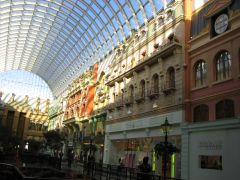
\includegraphics[width=.45\linewidth]{gfx/example_1}} \quad
\subfloat[Pan ma signo.]
{\label{fig:example-b}
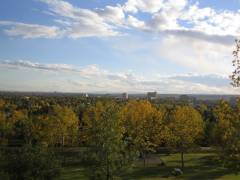
\includegraphics[width=.45\linewidth]{gfx/example_2}} \\
\subfloat[Methodicamente o uno.]
{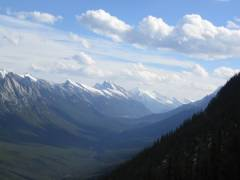
\includegraphics[width=.45\linewidth]{gfx/example_3}} \quad
\subfloat[Titulo debitas.]
{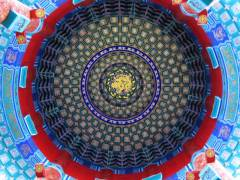
\includegraphics[width=.45\linewidth]{gfx/example_4}}
\caption[Tu duo titulo debitas latente]{Tu duo titulo debitas latente.}\label{fig:example}
\end{figure}
% Chapter 3

\chapter{Math Test Chapter} % Chapter title

\label{ch:mathtest} % For referencing the chapter elsewhere, use \autoref{ch:mathtest}

%----------------------------------------------------------------------------------------

\lipsum[13]

%----------------------------------------------------------------------------------------

\section{Some Formulas}

Due to the statistical nature of ionisation energy loss, large fluctuations can occur in the amount of energy deposited by a particle traversing an absorber element\footnote{Examples taken from Walter Schmidt's great gallery: \\ \url{http://home.vrweb.de/~was/mathfonts.html}}.  Continuous processes such as multiple scattering and energy loss play a relevant role in the longitudinal and lateral development of electromagnetic and hadronic showers, and in the case of sampling calorimeters the measured resolution can be significantly affected by such fluctuations in their active layers.  The description of ionisation fluctuations is characterised by the significance parameter $\kappa$, which is proportional to the ratio of mean energy loss to the maximum allowed energy transfer in a single collision with an atomic electron: \graffito{You might get unexpected results using math in chapter or section heads. Consider the \texttt{pdfspacing} option.}
\begin{equation}
\kappa =\frac{\xi}{E_{\mathrm{max}}} %\mathbb{ZNR}
\end{equation}
$E_{\mathrm{max}}$ is the maximum transferable energy in a single collision with an atomic electron.
\[E_{\mathrm{max}} =\frac{2 m_{\mathrm{e}} \beta^2\gamma^2 }{1 + 2\gamma m_{\mathrm{e}}/m_{\mathrm{x}} + \left ( m_{\mathrm{e}} /m_{\mathrm{x}}\right)^2}\ ,\]
where $\gamma = E/m_{\mathrm{x}}$, $E$ is energy and $m_{\mathrm{x}}$ the mass of the incident particle, $\beta^2 = 1 - 1/\gamma^2$ and $m_{\mathrm{e}}$ is the electron mass. $\xi$ comes from the Rutherford scattering cross section and is defined as:
\begin{eqnarray*} \xi  = \frac{2\pi z^2 e^4 N_{\mathrm{Av}} Z \rho
\delta x}{m_{\mathrm{e}} \beta^2 c^2 A} =  153.4 \frac{z^2}{\beta^2}
\frac{Z}{A}
\rho \delta x \quad\mathrm{keV},
\end{eqnarray*}
where

\begin{tabular}{ll}
$z$ & charge of the incident particle \\
$N_{\mathrm{Av}}$ & Avogadro's number \\
$Z$ & atomic number of the material \\
$A$ & atomic weight of the material \\
$\rho$ & density \\
$ \delta x$ & thickness of the material \\
\end{tabular}

$\kappa$ measures the contribution of the collisions with energy transfer close to $E_{\mathrm{max}}$.  For a given absorber, $\kappa$ tends towards large values if $\delta x$ is large and/or if $\beta$ is small.  Likewise, $\kappa$ tends towards zero if $\delta x $ is small and/or if $\beta$ approaches $1$.

The value of $\kappa$ distinguishes two regimes which occur in the description of ionisation fluctuations:

\begin{enumerate}
\item A large number of collisions involving the loss of all or most of the incident particle energy during the traversal of an absorber.

As the total energy transfer is composed of a multitude of small energy losses, we can apply the central limit theorem and describe the fluctuations by a Gaussian distribution. This case is applicable to non-relativistic particles and is described by the inequality $\kappa > 10 $ (\ie, when the mean energy loss in the absorber is greater than the maximum energy transfer in a single collision).

\item Particles traversing thin counters and incident electrons under any conditions.

The relevant inequalities and distributions are $ 0.01 < \kappa < 10 $, Vavilov distribution, and $\kappa < 0.01 $, Landau distribution.
\end{enumerate}

%----------------------------------------------------------------------------------------

\section{Various Mathematical Examples}

If $n > 2$, the identity \[t[u_1,\dots,u_n] = t\bigl[t[u_1,\dots,u_{n_1}], t[u_2,\dots,u_n] \bigr]\] defines $t[u_1,\dots,u_n]$ recursively, and it can be shown that the alternative definition \[t[u_1,\dots,u_n] = t\bigl[t[u_1,u_2],\dots,t[u_{n-1},u_n]\bigr]\] gives the same result.



\cleardoublepage % Empty page before the start of the next part

%----------------------------------------------------------------------------------------
%	THESIS CONTENT - APPENDICES
%----------------------------------------------------------------------------------------

\appendix

\part{Appendix} % New part of the thesis for the appendix

% Appendix A

\chapter{Appendix Test}

%----------------------------------------------------------------------------------------

\lipsum[13-14]

%----------------------------------------------------------------------------------------

\section{Appendix Section Test}
\lipsum[15]

\graffito{More dummy text}
\lipsum[16]

%----------------------------------------------------------------------------------------

\section{Another Appendix Section Test}
\lipsum[17]

\begin{table}
\myfloatalign
\begin{tabularx}{\textwidth}{Xll} \toprule
\tableheadline{labitur bonorum pri no} & \tableheadline{que vista}
& \tableheadline{human} \\ \midrule
fastidii ea ius & germano &  demonstratea \\
suscipit instructior & titulo & personas \\
\midrule
quaestio philosophia & facto & demonstrated \\
\bottomrule
\end{tabularx}
\caption[Autem usu id]{Autem usu id.}
\label{tab:moreexample}
\end{table}

\lipsum[18]

There is also a useless Pascal listing below: \autoref{lst:useless}.

\begin{lstlisting}[float=b,language=Pascal,frame=tb,caption={A floating example (\texttt{listings} manual)},label=lst:useless]
for i:=maxint downto 0 do
begin
{ do nothing }
end;
\end{lstlisting} % Appendix A
%% Appendix X

\chapter{Appendix Title}

%----------------------------------------------------------------------------------------

% Content begins here % Appendix B - empty template

%----------------------------------------------------------------------------------------
%	POST-CONTENT THESIS PAGES
%----------------------------------------------------------------------------------------

\cleardoublepage% Bibliography

\label{app:bibliography} % Reference the bibliography elsewhere with \autoref{app:bibliography}

\manualmark % Work-around to have small caps also here in the headline
\markboth{\spacedlowsmallcaps{\bibname}}{\spacedlowsmallcaps{\bibname}} % Work-around to have small caps also
%\phantomsection
\refstepcounter{dummy}

\addtocontents{toc}{\protect\vspace{\beforebibskip}} % Place the bibliography slightly below the rest of the document content in the table of contents
\addcontentsline{toc}{chapter}{\tocEntry{\bibname}}


\printbibliography
 % Bibliography

\cleardoublepage% Declaration

\refstepcounter{dummy}
\pdfbookmark[0]{Declaration}{declaration} % Bookmark name visible in a PDF viewer

\chapter*{Declaration} % Declaration section text

\thispagestyle{empty}

Put your declaration here.
\bigskip
 
\noindent\textit{\myLocation, \myTime}

\smallskip

\begin{flushright}
\begin{tabular}{m{5cm}}
\\ \hline
\centering\myName \\
\end{tabular}
\end{flushright}
 % Declaration

\cleardoublepage% Colophon (a brief description of publication or production notes relevant to the edition)

\pagestyle{empty}

\hfill

\vfill

\pdfbookmark[0]{Colophon}{colophon}

\section*{Colophon}

This document was typeset using the typographical look-and-feel \texttt{classicthesis} developed by Andr\'e Miede. The style was inspired by Robert Bringhurst's seminal book on typography ``\emph{The Elements of Typographic Style}''. \texttt{classicthesis} is available for both \LaTeX\ and \mLyX: 

\begin{center}
\url{https://bitbucket.org/amiede/classicthesis/}
\end{center}

\noindent Happy users of \texttt{classicthesis} usually send a real postcard to the author, a collection of postcards received so far is featured here: 

\begin{center}
\url{http://postcards.miede.de/}
\end{center}
 
\bigskip

\noindent\finalVersionString % Colophon

%----------------------------------------------------------------------------------------

\end{document}
